\documentclass[a4paper]{article}
\usepackage{graphicx}

\begin{document}

	\title{\Huge{Software Requirement Specification}}
	\author{Group 8}
	\maketitle

	\section{Introduction}

		Introduction

	\section{Vision}

		Vision

	\section{Background}

		Background

	\section{Architectural Requirements}

		\subsection{Access Channel Requiremnets}

			\begin{itemize}

				\item{An Item}

				\item{Another Item}

			\end{itemize}

		\subsection{Quality Requirements}

			\begin{enumerate}

				\item{An Item}

				\item{Another Item}

			\end{enumerate}

		\subsection{Integration Requirements}

			\begin{description}

				\item[first]{An Item}

				\item[second]{Another Item}

			\end{description}

		\subsection{Architecture Constraints}
		
			\subsubsection{Technologies}
		
				\begin{itemize}

					\item{Client interface must run on an Android device}

					\item{Client interface must be accessible through a web browser}
					
					\item{MySQL database must be used to store application data}
					
					\item{Python must be used in order to accommodate existing systems}

				\end{itemize}
				
			\subsubsection{Frameworks}
			
				\begin{itemize}

					\item{The application must be able to interface with the Django framework}

				\end{itemize}

	\section{Functional Requirements}

		\subsection{Introduction}

			This section introduces the functional requirements of the system, as seen by the different stakeholders:

			\subsubsection{Student}
				\begin{flushleft}
				A person who participates in examinable activities, for whom marks are recorded in the system. \linebreak 
				
				Students can:
				\end{flushleft}
				\begin{itemize}

					\item{View Marks}

				\end{itemize}

			\subsubsection{Marker}
				\begin{flushleft}
				A person who is responsible for grading a student, and who has to record marks for all students who he/she has graded. \linebreak 
				
				Markers can:
				\end{flushleft}
				\begin{itemize}

					\item{Input student marks}
					
					\item{View session marks}
					
					\item{Search for student}

				\end{itemize}
				
			\subsubsection{Lecturer}
				\begin{flushleft}
				A person who is responsible for setting examinable activities, as well as the logistics and administration of a particular course. \linebreak 
				
				Lecturers can:
				\end{flushleft}
				\begin{itemize}

					\item{Edit student marks}
					
					\item{View all marks}
					
					\item{Search for student}
					
					\item{Generate reports}
					
					\item{Assign system functions to Markers}
					
					\item{Create and edit marksheets}

				\end{itemize}
			
		\subsection{Scope and Limitations/Exclusions}
			\begin{figure}[h]
				\caption{High Level Use Case Diagram}
				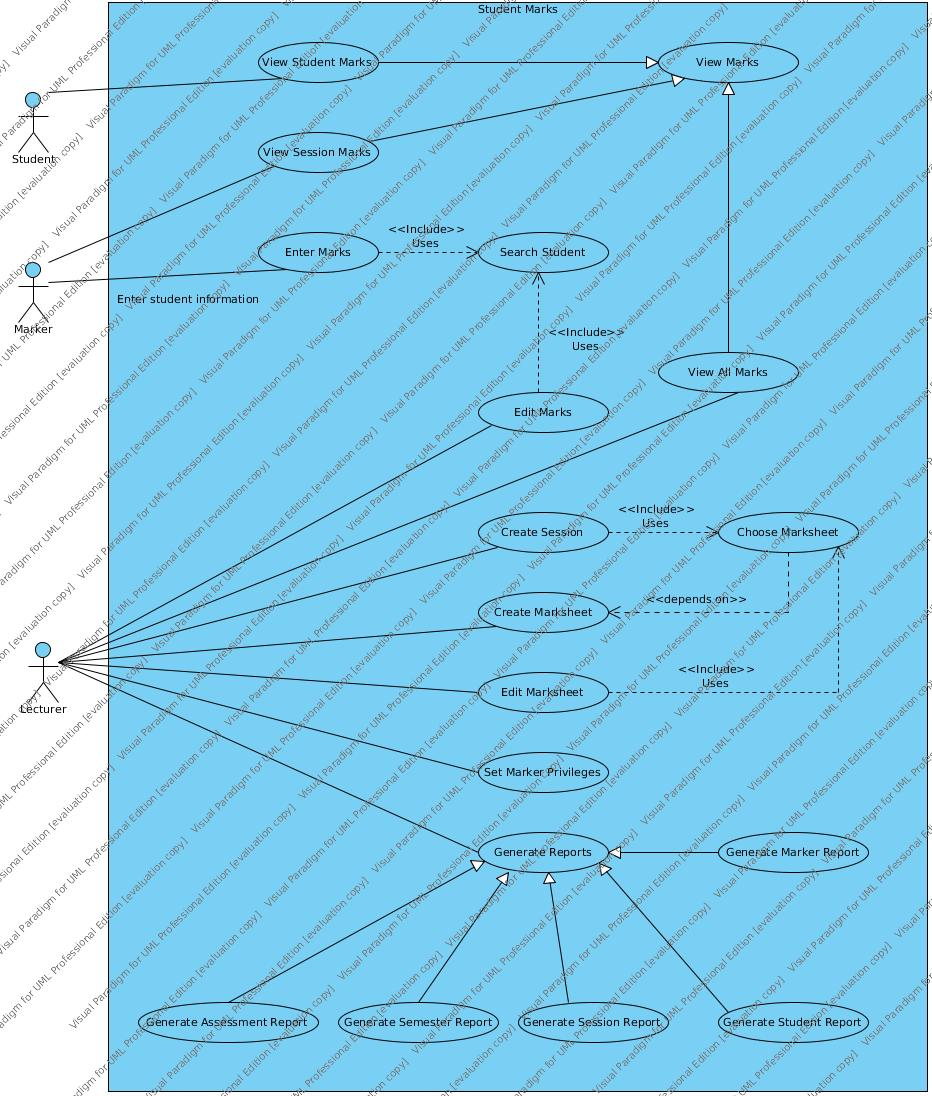
\includegraphics[height=10cm]{StudentMarks}
			\end{figure}

		\subsection{Required Functionality}

		\subsection{Use Case Prioritisation}

		\subsection{Use Case/Service Contracts}

		\subsection{Process Specification}

		\subsection{Domain Objects}

	\section{Open Issues}

	\section{Glossary}

\end{document}